\setcounter{secnumdepth}{3}
\chapter{Introduction}
\label{introduction}
\thispagestyle{plain}

Many people believe that AI (Artificial Intelligence) was created to imitate human behavior and the way humans think and act. Even though people are not wrong, AI was also created to solve problems that humans are unable to solve, or to solve them in a shorter amount of time, with a better solution. Humans may take days to find a solution, or may not find a solution at all that fits their needs. Search algorithms may deliver a very good solution in minutes, hours or days, depending on how much time the human is willing to use in order to get a better solution. \\
\\
%%%%%%%%%%%%%%%
A concrete example is the creation of timetables. Timetables can be used for educational purposes, sports scheduling, transportation timetabling, among other applications. The timetabling problem consists in scheduling a set of events (e.g., exams, people, trains) to a specified set of time slots, while respecting a predefined set of rules. These rules are called constraints in the timetabling subject, making harder to achieve a solution for the problem. In some cases the search space is so limited by the constraints that one is forced to "relax" them in order to find a solution. \\
\\
%%%%%%%%%%%%%%%
Solutions can be divided in multiple types, like \textit{feasible solutions}, \textit{non feasible solutions}, \textit{optimal solutions} or \textit{sub-optimal solution}. A feasible solution is a solution that solves all the mandatory problem constraints, in contrary to non feasible solutions. An optimal solution is the best feasible solution possible considering the problem and its optimal solution value. It's possible for a problem to have multiple optimal solutions. For last, non-optimal solutions are feasible solutions that can't reach the optimal solution value and so are not as good compared to an optimal solutions.\\
\\
%%%%%%%%%%%%%%%
The process of creating a timetable requires that the final solution follows a set of constraints. These can be divided in two groups: \textit{hard constraints} and \textit{soft constraints}. Hard constraints are a set of rules which must be followed in order to get a feasible solution. On the other hand, soft constraints represent the views of the different interested parties (e.g. institution, students, nurses, train operators) in the produced timetable. The satisfaction of these type of constraints is not mandatory as is the case of the hard constraints. In the timetabling problem, the goal is usually to optimize a function comprehending a weighted combination of the different soft constraints, while satisfying the set of hard constraints. \\
\\
%%%%%%%%%%%%%%%
The goal of the present project is to create an examination timetable generator using the ITC 2007 (International Timetabling Competition) specification. The solutions will be validated using a validator developed for this purpose in order to assess the quality of the solution. It is also required that the developed prototype may work with two exam epochs which can be considered an extension to the ITC-2007 formulation. In the end an (optional) Graphical User Interface will be created in order to allow the user to edit the current solution to fit the users needs and and to allow the optimization of the edited solution. The generator will be tested using data from ITC-2007 and some actual data from six different programs lectured at ISEL.
%%%%%%%%%%%%%%%
\section{Examination timetabling: State of the Art}
\label{sec:sota}
In this Section, we review the state of the art of problem at hand. We start by describing why timetabling is a rather complex problem, some possible approaches on trying to solve the problem and some of the solutions already taken, specifically for ITC 2007 data.
\\
%%%%%%%%%%%%%%%%%%%%
\subsection{Timetabling Problem}
%%%%%%%%%%%%%%%%%%%%
Timetabling is a subject that has been a target of research for about 50 years. Its problem may be formulated as a search or optimization problem (REF: 1999 Schaerf). As a search problem, the goal consist on finding a solution (feasible solution) that satisfies all the hard constraints, while ignoring the soft constraints. On the contrary, posing the timetabling problem as an optimization problem, one wants to find the best solution possible with time constraints. That is, one seeks to minimize (considering a minimization problem) the violations of soft constraints while satisfying the hard
constraints. Typically, the optimization is done after using a search procedure for finding an initial feasible solution.
\\
%%%%%%%%%%%%%%%
The basic examination timetabling problem, where only the clash hard constraint is observed, reduces to the graph coloring problem [ref.]. 
[Definir, resumidamente, o graph coloring problem.]
This is a well studied hard problem. Deciding whether a solution exists in the Graph Coloring problem is a NP-complete problem [ref. Arora and Barak book titled "Computational Complexity"]. Considering the graph coloring as an optimization problem, it is proven that the task of finding the optimal solution is a NP-Hard problem [ref. Arora and Barak book titled "Computational Complexity"].
\\
%%%%%%%%%%%%%%%%%%%%
\subsection{Existing approaches}
\label{subsection:ExistingAppr}
%%%%%%%%%%%%%%%%%%%%
Timetabling solution approaches are usually divided in the following categories [REF: survey R. Qu]: \textit{exact algorithms} (Branch-and-Bound, Dynamic Programming), \textit{graph based sequential techniques} (Saturation degree, Colour degree, Largest degree), \textit{local search based techniques} (Tabu Search, Simulated Annealing (SA), \textit{population based algorithms} (Evolutionary Algorithms, Memetic algorithms, Ant algorithms, Artificial immune algorithms), \textit{Multi-criteria techniques}, \textit{Hyper-heuristics}, \textit{Decomposition/clustering techniques} and \textit{hybrid algorithms}, which combine features of several algorithms, comprise the state-of-the-art. Due to its complexity, approaching the examination timetabling problem using exact method approaches can only be done for small size instances. Real problem instances found in practice are usually of large size, making the use of exact methods impracticable. Heuristic solution algorithms have usually employed to solve this problem.

Real problem instances are usually solved by using both Heuristics and Meta-heuristics algorithms. Heuristic algorithms are problem-dependent, meaning that these are adapted to a specific problem in which take advantage of its details. Heuristics are used to generate a feasible solution, focusing on solving all hard constraints only. Meta-heuristics on the other hand are problem-independent. These are used to, given the feasible solution obtained using heuristic algorithms, generate a better solution focusing on solving as many soft constraints as possible.\\
\\
Most of the Meta-heuristic algorithms used belong to one of the three categories: One-Stage algorithms, Two-Stage algorithms and Algorithms that allow relaxations. (REF: 2008 - Rhydian Lewis). 
\begin{itemize}
  \item The One-Stage algorithm is used to get an initial optimal solution, which the goal is to satisfy both hard and soft constraints at the same time. Approaches using this stage are not very common because it's hard to get proper solutions in a reasonable amount of time trying to satisfy both types of constraints at the same time;
  \item The Two-Stage algorithms are the most used types of approaches because is is divided in two phases (the reason for "Two-Stage" name). The first phase consists in all soft constraints being "discarded" and focus only on solving hard constraints to obtain a feasible solution. The next phase is an attempt to find the best solution, trying to solve the highest number of soft constraints possible given the solution of the first phase.
\end{itemize}

\subsubsection{Exact methods}
Some approaches may use \textit{exact methods} which may be viewed as tree algorithms and can be proved that it can find the optimal solution (global optimal). Exact methods search for solutions in the whole search space, and they divide the global problem into simpler problems in order to find the solution. This is not always used because these methods require a lot of computing time and they rarely produce results in a reasonable time in complex problems. Some approaches use some of these exact methods, namely: Constraint Programming Based Technique, Integer Linear Programming.\\

\paragraph{Constraint Programming Based Technique}
The Constraint Programming Based Technique (CPBT) allows direct programming with constraints which gives ease and flexibility in solving problems like timetabling. Two important features about this technique are backtracking and logical variables that facilitate searching for an optimal solution at the expense of time. Constraint programming is different from other types of programming, as in these types it is specified the steps that need to be executed, but in constraint programming it is specified the properties (hard constraints) of the solution or properties that should not be in the solution. [REF: 2009 - Qu Burke)]\\

\paragraph{Integer Linear Programming}
The Integer Linear Programming (ILP) is a mathematical programming technique in which the optimization problem to be solved must be formulated as an Integer Linear Problem, that is, the objective function and the constraints must be linear, and all problem variables are integer valued. If there are some variables that are continuous and other are integer, then the problem is called Mixed-Integer Linear Programming (MILP). Schaerf [REF: 1999 - Schaerf] surveys some approaches using the MILP technique to school, course, and examination timetabling.

\subsubsection{Graph Coloring}
The usual approaches start with using heuristics of Graph Coloring to get an initial solution that in most cases is a local optimum. Graph Coloring itself is not an heuristic or meta-heuristic but a method that designates a problem and its variants.\\

\paragraph{Graph Coloring Problems}
The Graph Coloring (GC) algorithm is divided in two main sub-types, which are \textit{vertex coloring} and \textit{edge coloring}.
\begin{itemize}
  \item The vertex coloring algorithm's main goal is to, given a number of vertices and edges, color the vertexes so that no adjacent vertices have the same color. In this algorithm, it's best to find a solution with the lowest number of colors as possible. In examination timetable problem, a basic approach could be to represent the exams as vertices and the hard constraints as edges (considering this is search algorithm, it is good to use optimization algorithms to deal with soft constraints) so that exams with the same color, can be assign to the same timeslot. After coloring, it proceeds to assign the exams into timeslots considering the colors of the solution. (REF: 2009 - Qu Burke)
  \item The edge coloring algorithm's main goal is equivalent to the vertex coloring algorithm, but this one is about coloring edges, so that no adjacent edges have the same color. As vertex's algorithm, the least colors possible, the better the solution is.
\end{itemize}

Graph Coloring heuristics like Saturation Degree Ordering are very commonly used to get the initial solutions. Others like First Fit, Degree Based Ordering, Largest Degree Ordering, Incident Degree Ordering are also heuristic techniques for coloring graphs.\\

\paragraph{Saturation Degree Ordering}
The Saturation Degree Ordering heuristic colors the vertices with more constraints first. The coloring method is as follows: while choosing a vertice to color, the ones with higher saturation degree will be colored first. The saturation degree of one vertice is the number of differently colored vertices adjacent to this vertice or, in another words, the number of different colors of all adjacent vertices. In the case of a tie, the highest saturation vertice with higher number of adjacent vertices is chosen.

\subsubsection{Meta-heuristics}
Meta-heuristics, as mentioned above, usually provide good solutions for optimization problems. In timetabling problems, meta-heuristic algorithms are used to optimize the feasible solutions provided by heuristics, like the GC. Meta-heuristics are divided in two main sub-types, which are \textit{Single-solution meta-heuristics} and \textit{Population-based meta-heuristics}.[REF:El-Ghazali Talbi - METAHEURISTICS - From Design to Implementation]\\

\paragraph{Population-based meta-heuristics}
Population-based meta-heuristics' main goal is to modify and optimize multiple candidate solutions, maintaining the search focused in the whole space. This type of meta-heuristic is therefore exploration oriented. Some examples of this type are \textit{particle swarm}, \textit{evolutionary algorithms}, \textit{genetic algorithms}.[REF:El-Ghazali Talbi - METAHEURISTICS - From Design to Implementation].\\

\paragraph{Single-solution meta-heuristics}
Single-solution meta-heuristics' main goal is to modify and optimize one single solution, maintaining the search focused in local regions. This type of meta-heuristic is therefore exploitation oriented. Some examples of this type are \textit{SA}, \textit{local search}, \textit{neighborhood search}, \textit{guided local search}[REF:El-Ghazali Talbi - METAHEURISTICS - From Design to Implementation]. \\
\\
The common types of algorithms and how they are organized, are displayed in Figure ~\ref{fig:TypesAlgorithms}

\begin{figure}[h!]
 \centering
   
\includegraphics{./images/types_of_algorithms.png}
   \caption{Types of algorithms adapted from [REF:El-Ghazali Talbi - METAHEURISTICS - From Design to Implementation].}
   \label{fig:TypesAlgorithms}
\end{figure}


\subsubsection{Some approaches applied to the ITC 2007 Examination timetabling problem}
\label{subsection:ApprITC2007}

I will briefly describe some techniques used in ITC 2007 - Examination timetabling, as detailed explanations about its techniques are properly presented in its articles which will be referenced below. ITC 2007 Examination timetabling problem consists on submitting a solution which may solve all hard constraints and the quality of each solution is calculated using the soft constraints the the solution didn't solve. Each soft constraint has its weight in the problem's context, and that weight adds points to each other solution. In this case, the more points a solution has, the worse it is. Solutions with zero points are considered optimal solutions, because they were able to solve all hard and soft constraints. Each of these constraints are presented on ITC's site (REF: ITC's site) or it can be read in Tomas Muller's article as he explains each constraints, including for other educational timetabling problems, named \textit{post enrollment based course timetabling}, and \textit{curriculum based course timetabling}\\
\\

\paragraph{\textbf{Tomas Muller's approach:}}

Tomas Muller's approach was actually used to solve all three problems established by ITC 2007 competition. He was able to win two of them and be finalist on the third. For solving the problems, he opted for an hybrid approach. Meaning it has more than one algorithm working at the same time for first (construction) phase and/or for the second (optimization) phase. In this case, he chose to use multiple algorithms to optimize its first solutions.\\
\\
In the \underline{first phase}, Tomas used Iterative Forward Search algorithm (REF: Muller 2005) to obtain feasible solutions and Conflict-based Statistics (Muller et al. 2004) to prevent Iterative Forward Search from looping. \\
\\
Iterative Forward Search algorithm assigns a value to one unassigned variable on each iteration. These variables are exams (in examination timetabling problem) and are only assignable if the result won't cause violations of hard constraints. If it's the case, some precautions may be applied to continue with the algorithm. An assign will result in an exam (the variable assigned) being held in a room X, time Y with Z students. The variable chosen in each iteration is randomized or parameterized to, for example, assign the most difficult assignable exam first. The Conflict-based Statistics was used to memorize some previously passed conflicts and avoid repeating those for each iteration.\\
\\
The \underline{second phase} consists in using multiple optimization algorithms. These algorithms are applied using this order: Hill Climbing, edited Great Deluge (REF: Dueck 1993) and optionally Simulated Annealing (REF: Kirkpatrick et al. 1983).\\
\\
Hill Climbing is used to optimize the current solution only, by generating a neighbor solution each iteration. The neighbor solution is only accepted if the "score" of this solution is lower than the one we had before (only soft constraints count now) and no hard constraint is violated. If there is no better solutions for a number of iterations, which is parameterized, this algorithms stops running and the Great Deluge starts doing its job.\\
\\
Great Deluge, used after the solution cannot be improved using the previous algorithm. This method can be seen as a Hill Climbing variation, as it always accepts going up but is also able to go down the Hill as long as it doesn't go lower the water level. This means that it accepts worse neighbor solutions compared to the current solution, but only accepts worse solutions which absolute value is less compared to the value of the Bound, as the Bound is the variable that corresponds to the water level mentioned earlier. The water level is always going up, until reaching a local/global maximum. The initial Bound and the way the Bound decreases (water level going up) is parameterized.\\
\\
When Simulated Annealing (SA) is used (remember that this method is optional), it is used after Great Deluge reaches his bound lower limit. If this method is not meant to be used, Great Deluge might be running until reaches timeout or a global maximum. SA is a method similar to Hill Climbing, as it accepts neighbor solutions better than the current one. But this method also allows neighbor solutions that are worse than the current one, by establishing a mathematical operation using a variable called Temperature. The result of this operation stands for "how much wrong can the solution become" in order to avoid local maximums. This variable called Temperature is parameterized so as the Cooling Rate variable which is multiplied by the Temperature each iteration, in order to reduce the Temperature. This means that for each iteration, neighbor solutions will get less worse and it is possible to reach a local maximum again. If the local maximum is the same (solution is the same as before running Simulated Annealing), that means the maximum Temperature must get higher in order to avoid the local maximum and/or to possibly get a better solution. As the Temperature gets higher, Simulated Annealing is not repeated, but instead, Hill Climbing takes control again.\\
\\
This is the basics and a resume of Muller's approach. More detailed explanations and implementations can be viewed on this article (REF: 2009 - Thomas Muller - ITC2007 solver description a hybrid approach).\\
\\
\paragraph{\textbf{Christos Gogos' approach:}}

Gogos was able to reach second place in Examination Timetabling, right after Muller. Gogos' approach is very different compared to Muller's. His approach, like Muller's, was divided in 2 phases named \textit{Construction Phase} and \textit{Improvement Phase}, which the first is to get a feasible solution and the second is to improve the solution found in the first phase, using local search algorithms.\\
\\
In the \underline{first phase}, is starts using a Pre-processing stage. It is called \textit{Pre-processing} because it's a stage that adds additional information to the main problem in order to make it easier to handle in the further steps. This stage deals with hidden dependencies, which means it adds dependencies to the problem that weren't there in the beginning but they exist and makes sense in the problem itself. For example, one hidden dependency may be one exam E1 having an ordering constraint with exam E2 stating that E2 must be scheduled after exam E1 and exam E3 must be scheduled after exam E2. So a dependency/constraint must be added so exam E3 must be scheduled after exam E1 as well. Gogos believes that this pre-process method will be very helpful in the further stages when trying to find solutions.\\
\\
After the pre-processing stage, a construction stage takes place. This method is used to create a complete timetable. In this stage, multiple solutions are attempted considering the available time in which only the best solution is passed to the next phase. The solution is constructed by constantly setting an exam and a room to a period until a feasible solution is found. This selection is not random, instead some rules must be applied. This method however is not a very known or common algorithm.\\
\\
In the \underline{second phase}, Hill Climbing is used. This algorithm is used to get generate neighbor solutions, accepting only better solutions compared to the current one, until reaching a local maximum. It is considered local maximum when Hill Climbing cannot generate a better solution in a number amount of tries or time limit.\\
\\
Next stage consists in utilizing Simulated Annealing to get out of local maximum. Simulated Annealing skipped when it cannot generate better solutions after a set period of time.\\
\\
After Simulated Annealing, an Integer Programming formulation that uses Breach and Bound is used in a set of sub-problems. This stage is called "IP Sub-Problems Stage". This simply examines all periods trying to discover some possible improvements that can be done, for example, swapping a room with high penalty with a room with no or low penalty that is not currently being used.\\
\\
The last stage is the Shaking Stage. This method "shakes" the current best solution in order to get equally good solutions and pass it to Simulated Annealing stage. This method is not used if the problem we're solving only has 1 room or the cost of each room assign is zero. Two heuristics are used in this stage. The first creates neighbor solutions but a solution is only accepted if the new solution is equally good and the room arrangement is better (total cost of room assignment is lower) compared to the current best solution. The second heuristic reschedule a set of exams presented on the latest solution. These are first removed from the timetable and then scheduled using the same techniques used in the construction stage. This heuristic will probably generate a worse solution but it is accepted and used next on Simulated Annealing stage.\\
\\
Tabu Search is also used in this approach, even tho it's not used as a standalone method. This one is used along with Hill Climbing and Simulated Annealing algorithms to prevent them from looping and creating the same results. Tabu Search avoids the creation of equal neighbor solutions by not letting the same period be selected for swapping after this being selected once. This period can only be selected again after a certain number of swaps on other periods.\\
\\
This was a brief resume of Gogos' approach. Detailed explanations, implementations, experiments and results are present on this article (REF: 2010 - Gogos et al. - An improved multi-staged algorithmic process for the solution of the examination timetabling problem)\\
\\
It is possible to check the results of ITC 2007's Examination challenge in Figure~\ref{fig:Top5itc}, which illustrates these two top competitors on this challenge. Most of the test instances shows that Muller got the least points (black numbers and dots) and so the reason why he ended up winning. Gogo's results were a little worse (orange numbers and dots) compared to Muller's results and beat the other competitors in most of the instances, not including instances 10 and 12 which no valid solutions were found. Calculating the instance's points, Gogo ended up in second place. All the results can be seen on ITC's original site (REF: ITC's site with results) or on Muller's article (REF: 2009 - Thomas Muller - ITC2007 solver description a hybrid approach)

\begin{figure}[h!]
 \centering
   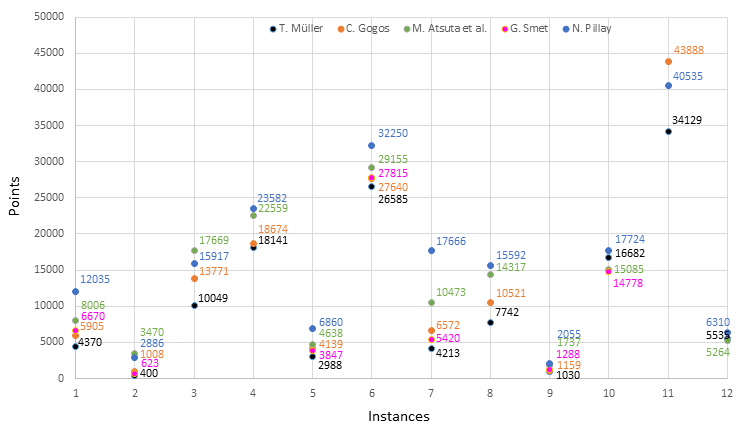
\includegraphics[scale=1]{./images/presentation.png}
   \caption{Top 5 results on ITC 2007 Examination Challenge}
   \label{fig:Top5itc}
\end{figure}




%%%%%%%%%%%%%%%%%%%%%%%%%%%%%%%%%%%%%%%%%%

\iffalse
Another tourist guide application with some interesting features is the GuidePal Offline City Guides~\cite{GuidePalWeb}\cite{GuidePaliPhone}. It allows users to download varied content for different cities and to consult information regarding restaurants, coffee shops, places to visit, and other attractions. Two screenshots of this application are illustrated on Figure~\ref{fig:guidePalIphoneScreenshots}.\\
\\
\begin{figure}
        \centering
        \begin{subfigure}[b]{0.25\textwidth}
                \centering
                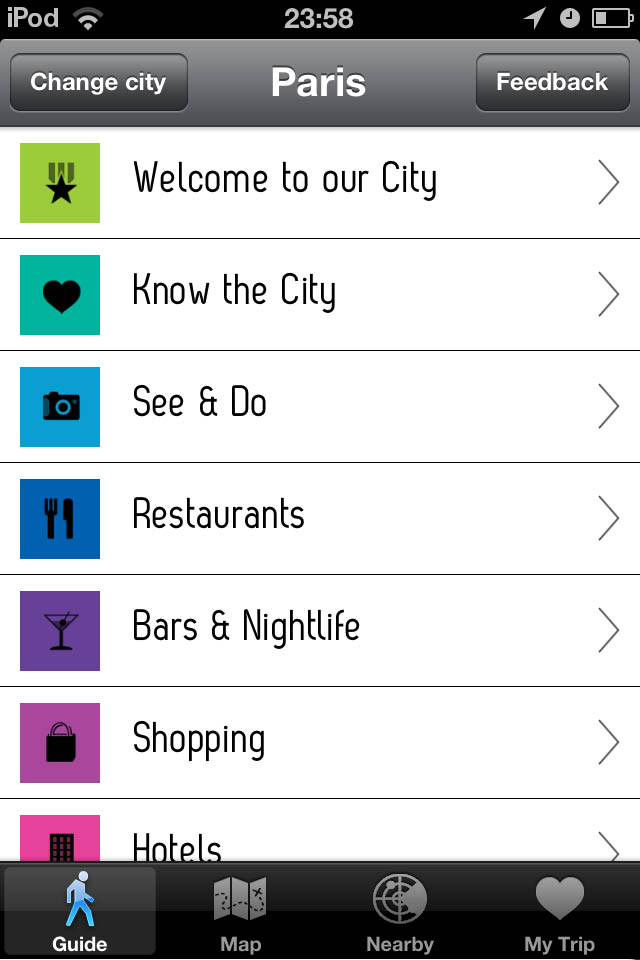
\includegraphics[height=7.5cm]{./images/screenshots/screenshot_guidepal_1.jpg}
                \caption{Category selection for filtering the locations.}
                \label{fig:guidePalCategorySelection}
        \end{subfigure}%
        \quad\quad\quad\quad\quad
        \begin{subfigure}[b]{0.25\textwidth}
                \centering
                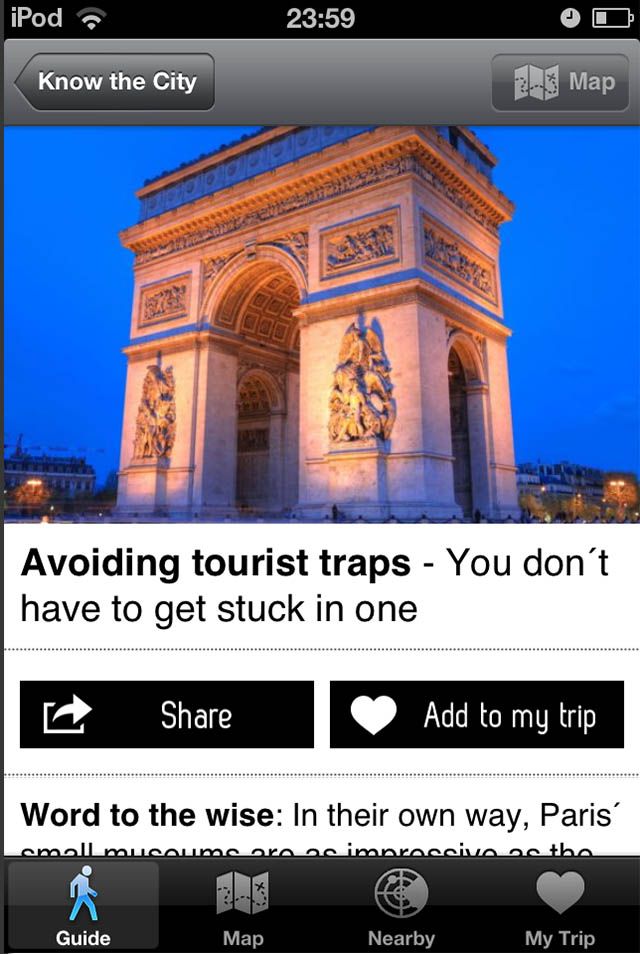
\includegraphics[height=7.5cm]{./images/screenshots/screenshot_guidepal_2.jpg}
                \caption{Detailed information about touristic location.}
                \label{fig:guidePalDetailedInformation}
        \end{subfigure}
        \caption{GuidePal~\cite{GuidePalWeb}\cite{GuidePaliPhone} iPhone application screenshots.}
        \label{fig:guidePalIphoneScreenshots}
\end{figure}
\\
In order to list the existing points of interest, the user selects the desired city and category as illustrated by  Figure~\ref{fig:guidePalIphoneScreenshots}~(\subref{fig:guidePalCategorySelection}). After selecting the intended category, a description for the point of interest is presented; Figure~\ref{fig:guidePalIphoneScreenshots}~(\subref{fig:guidePalDetailedInformation}) shows the selection of the "Know the City" category.\\
\\
This application also have some augmented reality features, providing users with the possibility to map the real world (captured by the camera of the device) with the touristic attractions in real time. When the camera points to the direction where touristic locations are available near by, those are presented above the image. By selecting any of the presented locations, the user is redirected to the detail page similar to one illustrated on Figure~\ref{fig:guidePalIphoneScreenshots}~(\subref{fig:guidePalDetailedInformation}).
%%%%%%%%
\subsection{mTrip}
mTrip~\cite{mTrip} travel guide service is mainly used for big cities such as Paris, Berlin,  Madrid, and others. It is available as a separate application for each one of the major cities (for both iPhone and Android) and allows people to consult information regarding points of interest without an Internet connection. Figure~\ref{fig:mtripScreenshots} presents some screenshots of this application. \\
\\
Users can plan an itinerary or create guides for the cities by providing the detailed information on the touristic attractions they plan to visit. After specifying the dates for the trip, each user can manually compose his itinerary or allow mTrip to automatically generate an itinerary for the trip. When the automatic mode is chosen, one must indicate preferences for the attractions to be visited, as shown on Figure~\ref{fig:mtripScreenshots}~(\subref{fig:mTripPreferencesCustomization}). A list of points of interest is presented when the user selects a specific category, similar to those shown on Figure~\ref{fig:mtripScreenshots}~(\subref{fig:mTripTouisticLocations}).
\\
%%%%%%%%%%%%%%%%%
\begin{figure}
        \centering
        \begin{subfigure}[b]{0.25\textwidth}
                \centering
                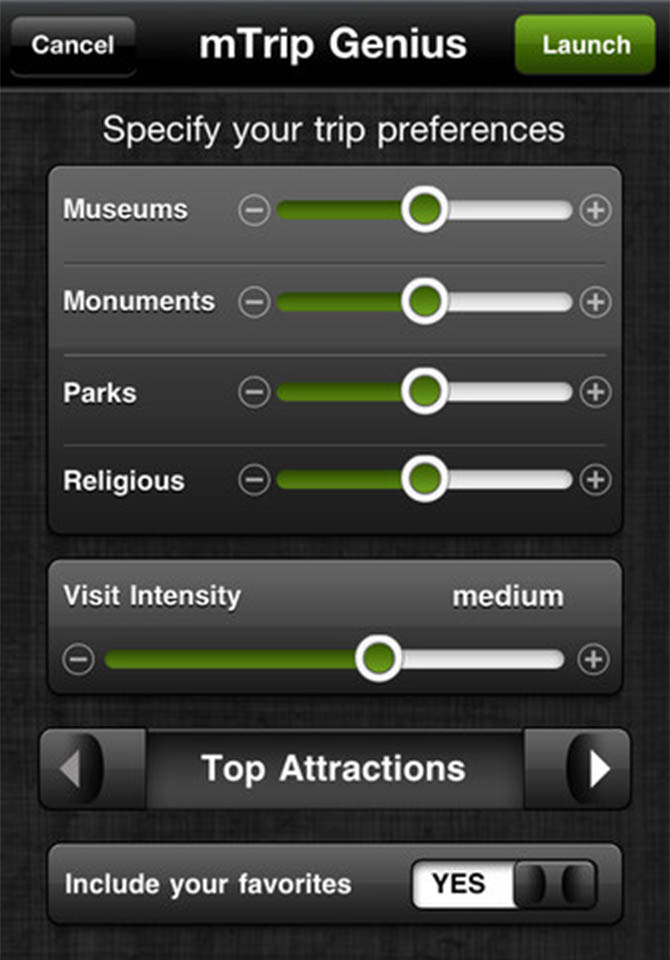
\includegraphics[height=7.5cm]{./images/screenshots/screenshot_mtrip_1.jpg}
                \caption{Customization of the itinerary.}
                \label{fig:mTripPreferencesCustomization}
        \end{subfigure}%
        \quad\quad\quad\quad\quad\quad
        \begin{subfigure}[b]{0.25\textwidth}
                \centering
                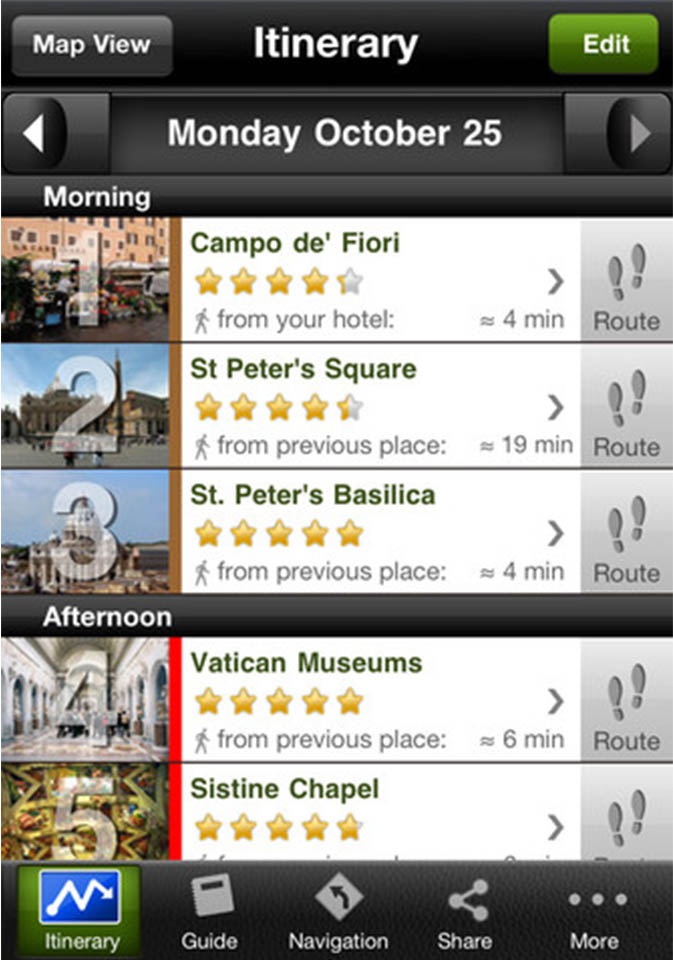
\includegraphics[height=7.5cm]{./images/screenshots/screenshot_mtrip_2.jpg}
                \caption{List of the touristic locations.}
                \label{fig:mTripTouisticLocations}
        \end{subfigure}
        \caption{mTrip iPhone application screenshots.}
        \label{fig:mtripScreenshots}
\end{figure}
\\
%%%%%%%%%%%%%%%%%
Each point of interest is accompanied by a description, a photo, opening hour, prices, as well as the comments and ratings from other travellers. The application provides an augmented reality tool that allows to preview of the points of interest around the user's current location.
%%%%%%%%
\subsection{Triposo}
Triposo~\cite{triposo} shares similar concepts with the mTrip application. However, it includes much more countries as well as smaller cities. When one picks the country to visit, the download of information regarding the points of interest for that country starts immediately, allowing to consult this information later in offline mode. Some major cities require additional downloads due to the large amount of the points of interest and touristic attractions. For big cities, users have access to special information regarding the city guide about all sights, a list of restaurants and extended nightlife options. The application also offers a travel dashboard with currency converter, weather, and useful native language phrases. Triposo uses freely available content from different sources, such as Wikipedia~\cite{wikipedia}, Wikitravel~\cite{wikitravel}, World66~\cite{world66}, among others.\\
\\
As it is shown by the screenshot on Figure~\ref{fig:triposoScreenshots}~(\subref{fig:triposoSuggestedPointsOfInterest}), a set of suggested points of interest for Lisbon is presented along with the main navigation items. Figure~\ref{fig:triposoScreenshots}~(\subref{fig:triposoWeahtherTime}) shows the current weather and current time for Porto as well as the spelling of some Portuguese words.\\
%%%%%%%%%%
\begin{figure}
        \centering
        \begin{subfigure}[b]{0.25\textwidth}
                \centering
                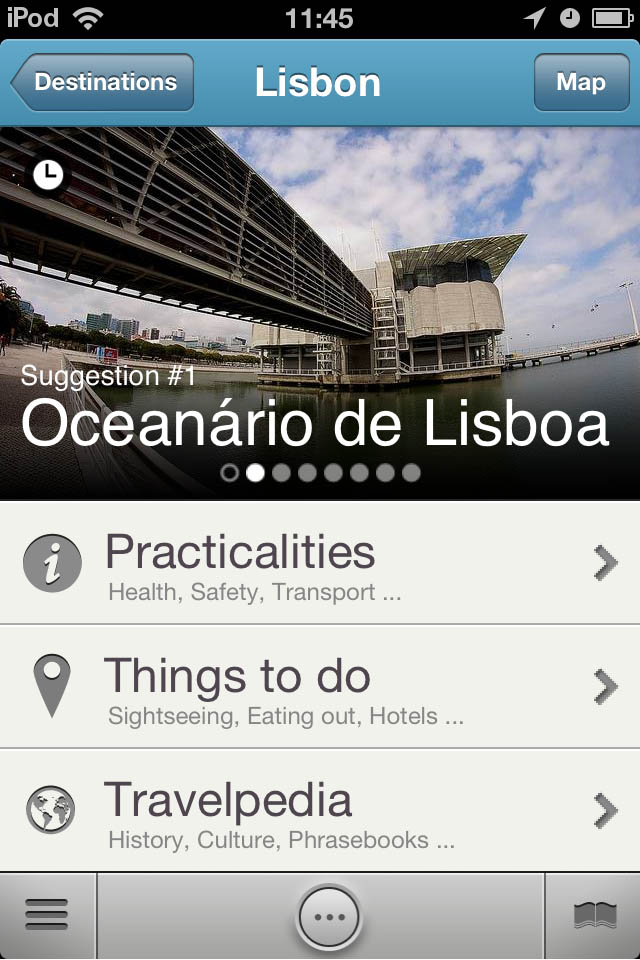
\includegraphics[height=7.5cm]{./images/screenshots/screenshot_triposo_1.jpg}
                \caption{Suggested points of interest.}
                \label{fig:triposoSuggestedPointsOfInterest}
        \end{subfigure}%
        \quad\quad\quad\quad\quad
        \begin{subfigure}[b]{0.25\textwidth}
                \centering
                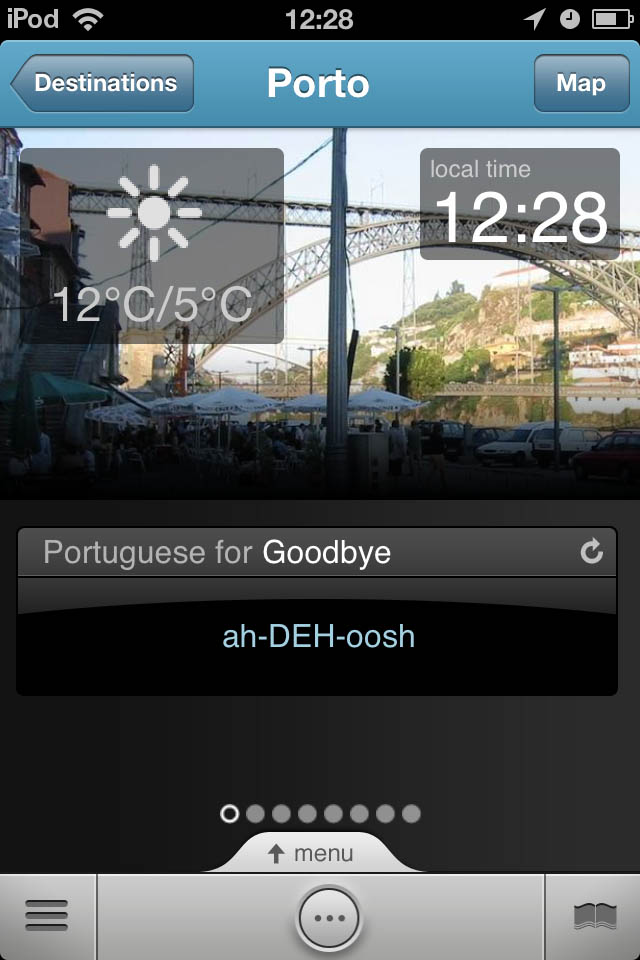
\includegraphics[height=7.5cm]{./images/screenshots/screenshot_triposo_2.jpg}
                \caption{Shortcuts and useful information.}
                \label{fig:triposoWeahtherTime}
        \end{subfigure}%
        \caption{Triposo iPhone application screenshots.}
        \label{fig:triposoScreenshots}
\end{figure}


%%%%%%%%%%
\subsection{Foursquare}
Foursquare is a service that allows registered users to "check-in\footnote{Check-in refers to the user's action for posting his current location at a venue.}" at their current location. It is composed by both web and mobile applications for iPhone, Android and Blackberry. Users with special permission have the possibility to contribute with new locations, such as coffee shops, restaurants, sights, among others. The service was created in 2009 and in March of 2011 a new version with a recommendation engine~\cite{foursqureRecommendationEngine} was developed, for suggesting places that users might like, based on their past actions.\\
\\
In 2013 an updated version of the service was launched, where users can consult the sights nearby their current location. The map view with the recommended sights nearby users current location is shown on Figure~\ref{fig:4SqureScreenshots}~(\subref{fig:4squre2}). An example of the touristic location details is shown on Figure~\ref{fig:4SqureScreenshots}~(\subref{fig:4squre3}) where user can have the preview of the location, save it to favourites, perform the check in, among others.\\
\\
\begin{figure}
        \centering
        \begin{subfigure}[b]{0.25\textwidth}
                \centering
                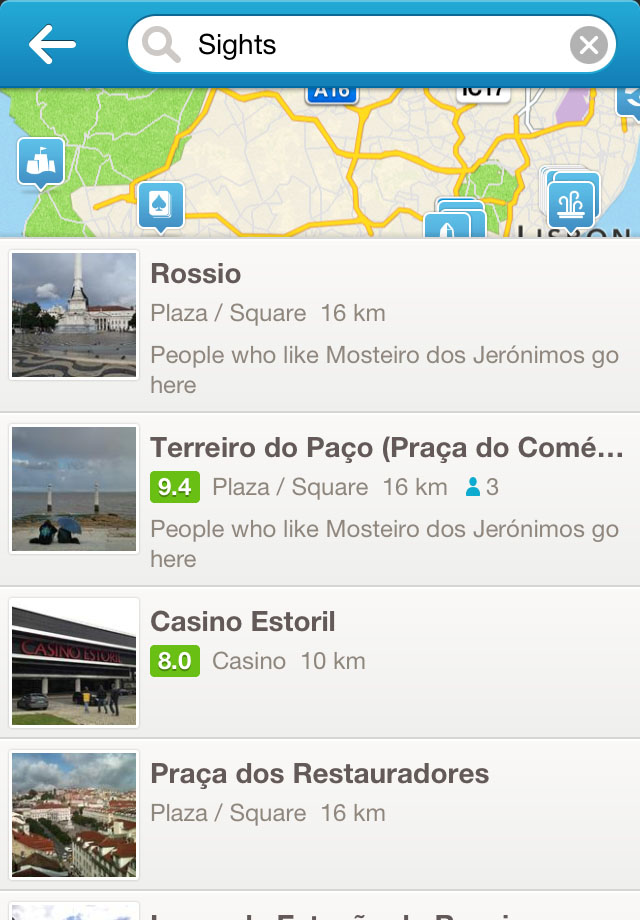
\includegraphics[height=7cm]{./images/screenshots/screenshot_foursqure_1.jpg}
                \caption{Map view with sights nearby user's location.}
                \label{fig:4squre2}
        \end{subfigure}%
        \quad\quad\quad\quad\quad
        \begin{subfigure}[b]{0.25\textwidth}
                \centering
                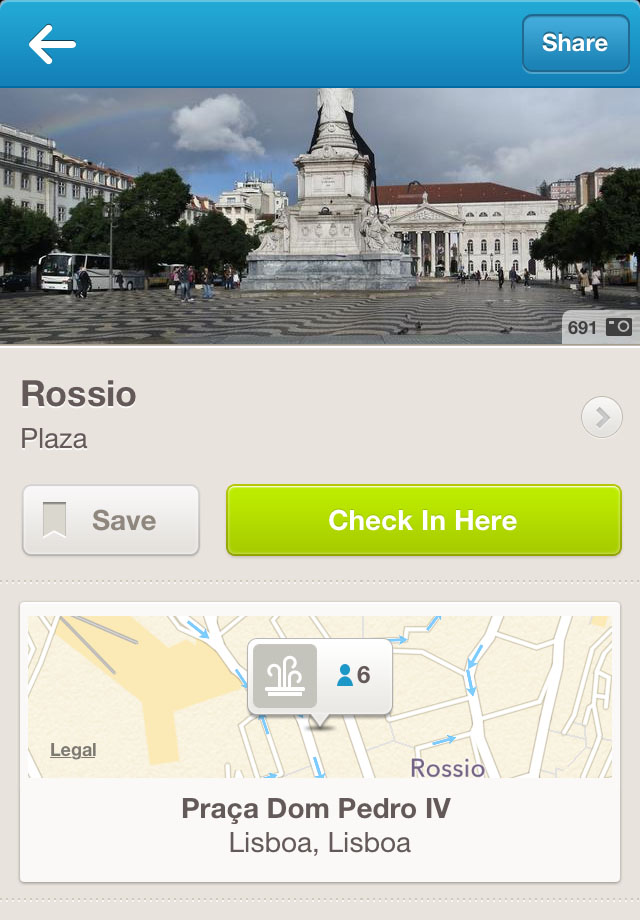
\includegraphics[height=7cm]{./images/screenshots/screenshot_foursqure_2.jpg}
                \caption{Details of the Touristic location.}
                \label{fig:4squre3}
        \end{subfigure}%
        \caption{Foursquare iPhone application screenshots.}
        \label{fig:4SqureScreenshots}
\end{figure}
\\
All these applications are modern solutions for tourist guides. The Foursquare service was created in 2009, the mTrip and TouristEye in 2010, whereas the Triposo and GuidePal have been published in 2011. 
\newpage

\section{Proposed Solution}
\label{sec:ftbd}
This Section introduces the simplified service architecture as well as the employed technologies used during the development of the system components. The system is mainly composed by the~\gls{rest}~\cite{RestWebber} service with a data access layer which exposes a set of endpoints\footnote{In \gls{soa}, an endpoint is the entry point to a service.} accessible by the client applications. Client applications are available as Web-based and Mobile (for iOS~\cite{ios} platforms iPhone and iPad). Figure~\ref{fig:introductioArchitecture} shows the proposed service architecture.\\
\\
\begin{figure}[h!]
 \centering
   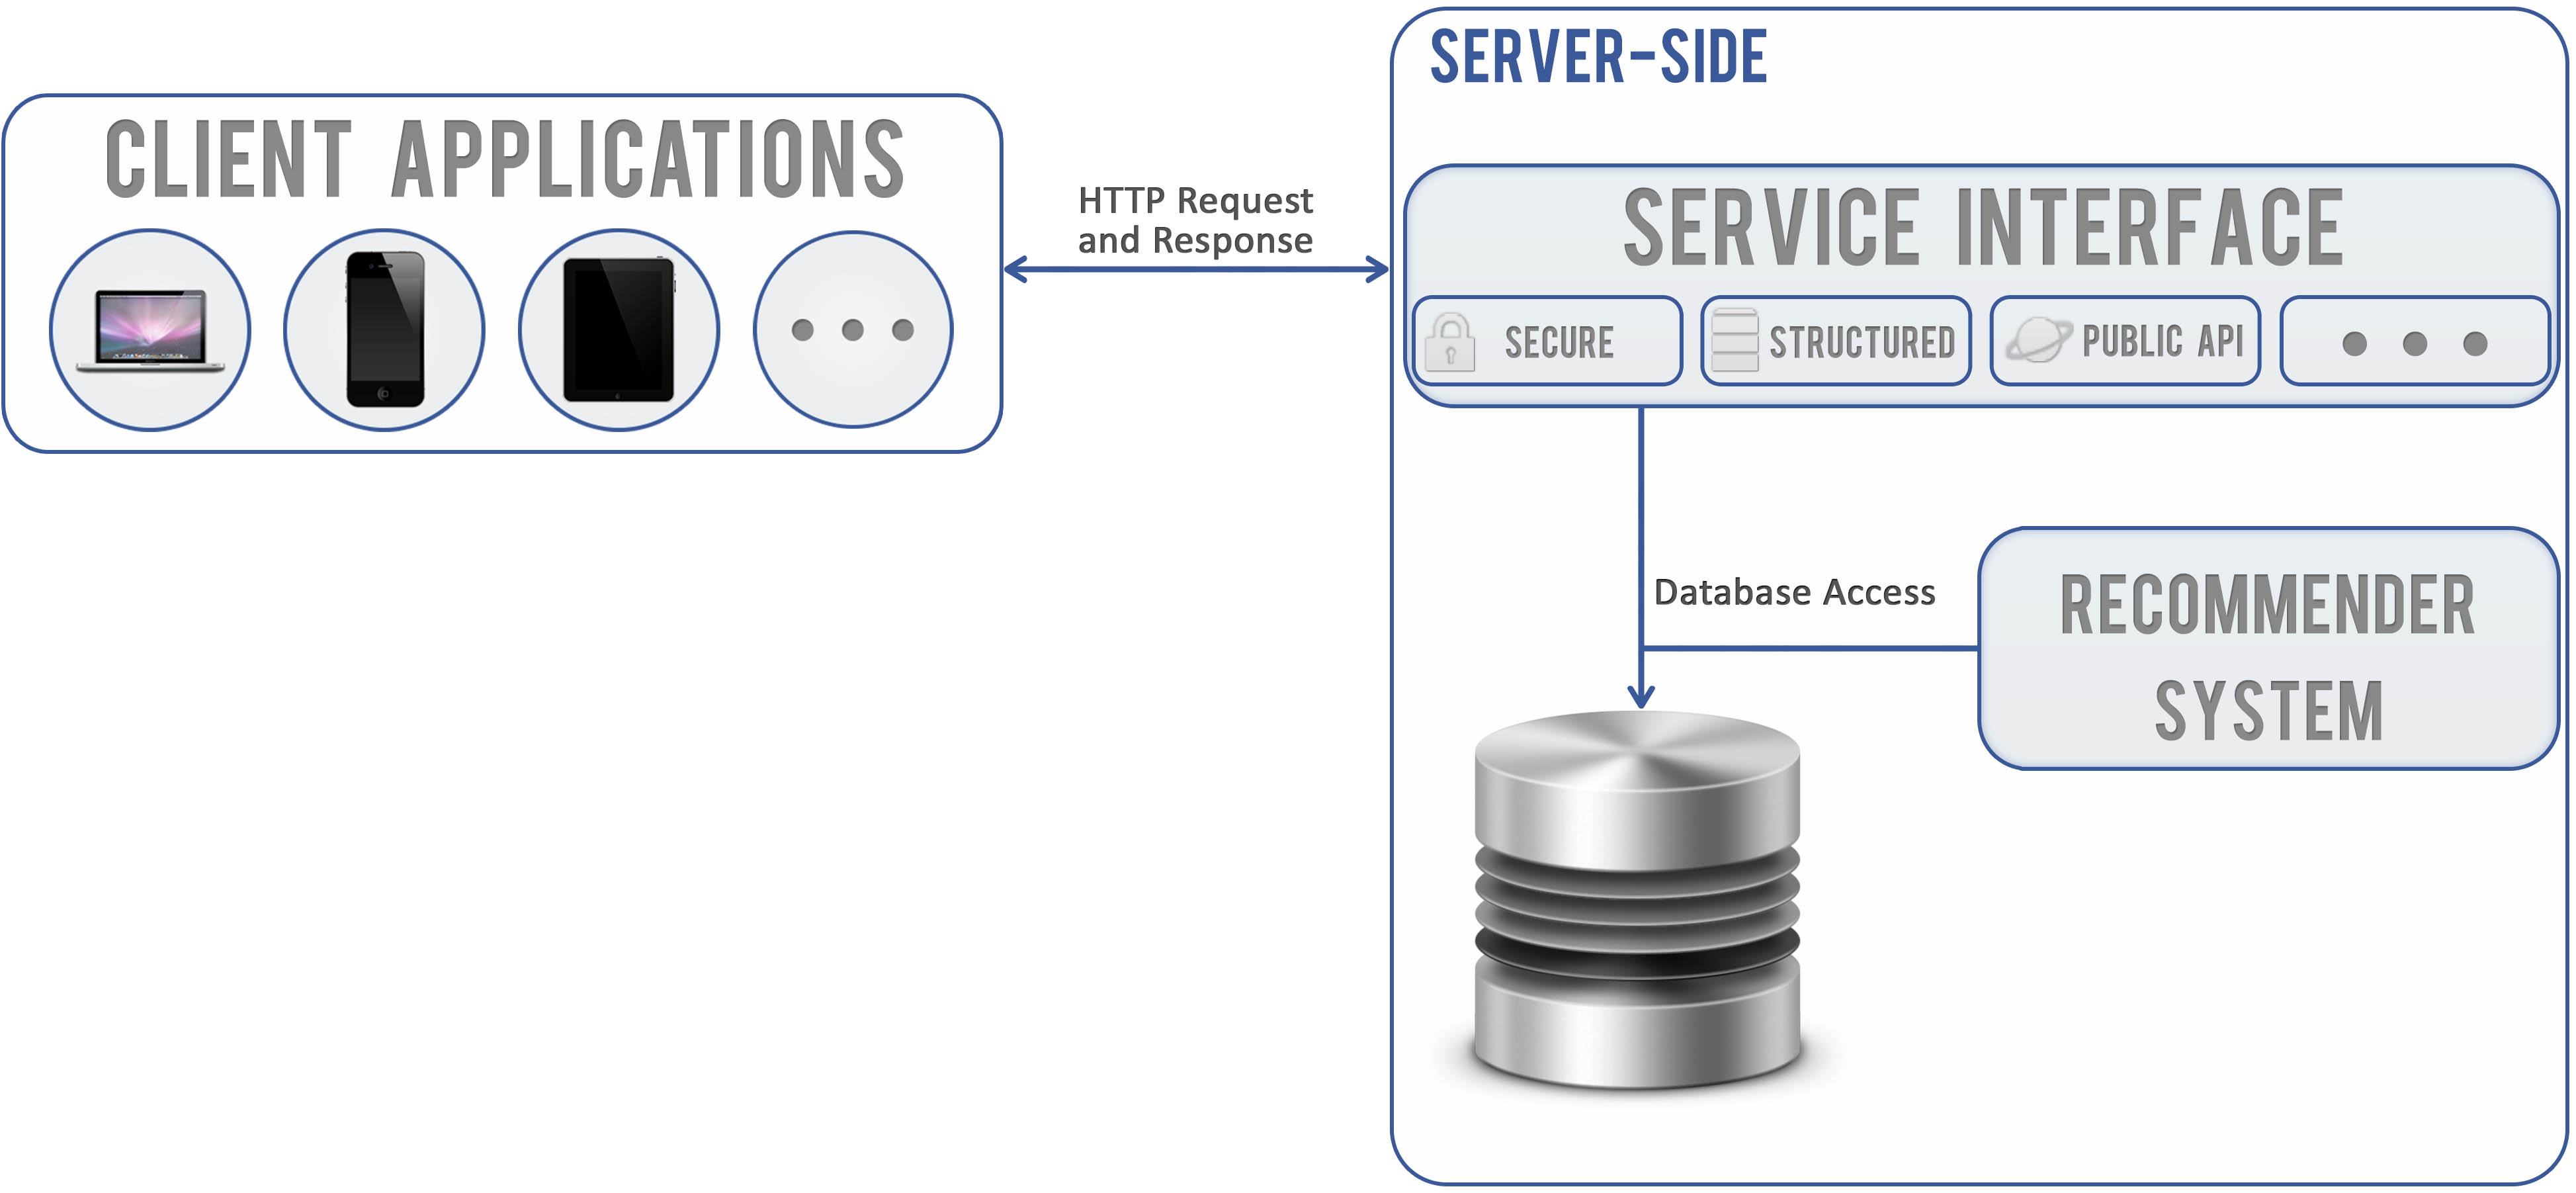
\includegraphics[width=14.8 cm]{./images/diagrams/diagram_introduction_architecture.jpg}
   \caption{Generic service architecture.}
   \label{fig:introductioArchitecture}
\end{figure}\\
\\
The service is divided into four main layers, with the following roles:
\begin{itemize}
 \item The Database layer stores information regarding points of interest, user data, among other types of data.
 \item The Service Interface is responsible for communicating with the Database layer. It makes all accesses transparent to the end client applications. This layer is mainly responsible for the data security and integrity, delivery of information in structured format, among others.
 \item The Recommender System is responsible for finding new points of interest based on the user's past actions, and to recommend these to the user. This service uses data from the database layer in order to compute recommendations.
 \item Client Applications make \gls{http} requests in order to access data from the public \gls{api}, provided by the Service Interface layer.
\end{itemize}

\subsection{Tools and Technologies}
\label{subsec:ttbuipd}
This Subsection introduces the technologies and tools used to achieve the goals of this project. We begin by describing a set of technologies related to databases, data model, and the \gls{rest} service. Then, the Web related technologies are discussed and finally we address the mobile applications.\\
\\
%%%%
For information storage, we use the MySQL~\cite{MySqlOrcale} relational database, which uses the \gls{sql} for accessing and manipulating databases. In order to facilitate the service development process, a pre-populated database was created with a few tens of points of interest.\\
\\
%%%%
The \gls{rest}~\gls{api} is developed in order to provide a single data source for client applications, including those already developed within this project and others that may appear in the future. The \gls{api} is implemented using the Java environment and Play~Framework~\cite{playFramework}.\\
\\
The Web application implementation is focused in technologies for user interface definition and structuring such as~\gls{html5}~\cite{html5},~\gls{css3}~\cite{css3} and also the JavaScript~\cite{javaScript} technology to enrich user's interactivity. The server side of the web application was developed using the Play Framework. Twitter Bootstrap~\cite{twitterBootstrap} framework was used to generate the layout with desired dynamic content, thus providing an user friendly platform.\\
\\
%\marginpar{} %%%
In the past few years, mobile devices have been used and widespread with great success, starting with Apple's iPhone launch and later with the iPad~\cite{iPadSanchez}. Both devices share the same operating system named iOS that offers a development platform for object-oriented applications. Those are written in Objective-C~\cite{ObjectiveC}\footnote{The Objective-C is a computer programming language based on C and Smalltalk. It is designed to leverage the C language with full object-oriented programming capability, through the mechanism of message passing. When in Objective-C one sends a message, its target is resolved at runtime and then it interprets the message with the receiving object~\cite{ObjectiveC}~\cite{objectiveCBook}.} using the iOS SDK (Software Development Kit). In the course of this project the targeted applications were designed taking into consideration advanced aspects of the iOS platform such as sharing code between iPhone and iPad, by means of an Universal Application~\cite{UniversalApps}.\\
\\
%\marginpar{} %%%
The development of these applications was carried out using the \gls{ide} Xcode~\cite{Xcode}.

\subsection{Core Features}
\label{subsec:cf}
This Subsection contains a description of the core features provided by the service, which are presented in Table~\ref{tab:coreFeatures}.\\
\\
\newpage
\begin{center}
    \begin{longtable}{ | p{3.5cm} | p{11.1cm} |}
    \caption{Core features of the GuideMe service.}
    \label{tab:coreFeatures}
	\\
    \hline
    \textbf{Feature Name} & \textbf{Description}\\ \hline
    \hline
    \specialcell[t]{Internationalization\\support} & 
    The aim of the project is to support points of interest of Portugal, but its architecture is designed in order to easily be expanded and to support other countries. Multilingual support is implemented for the database, REST API and application levels. \\ 
    \hline
    
    Filtering options &
    The following features are supported:
	\begin{itemize}
	\item lookup for points of interest nearby the user's current location;
	\item filtering of the locations based on the following characteristics:
	\begin{itemize}
		\item specific attraction;
		\item user's current location, by using the geographic coordinates retrieved from the mobile device;
		\item time that the user can spend;
		\item time of day of the visit;
		\item preferred weather conditions.
	\end{itemize}
	\item places that can be visited under given weather conditions such as rainy or sunny days, among others. It requires integration with the \gls{wwo} meteorology~\gls{api}, in order to advise or not the visit to the chosen user location;
	\item filtering by the maximum distance to the point of interest, based on the user's current location and mobility.
	\end{itemize}
    \\ 
    \hline
    
    \specialcell[t]{Wanted and\\already seen} &
	Users have the possibility to create a list of locations that they intend to visit as well as access the history of already visited locations. \\ 
    \hline

	\specialcell[t]{Social component} &
    	The following features are supported:
	\begin{itemize}
	\item Integration with social networks in order to encourage users to share visits with their friends;
	\item Based on the visits and mutual preferences between various users, the system recommends new places to visit that users may like. The recommendations are produced by the recommender system, using Collaborative Filtering (CF)~\cite{ibCollabrativeVSGK}\cite{AmazonRecommendGLBSJY}\cite{recommSystemPMVS} algorithms. The proposed solution is further explained in Section~\ref{sec:ocft};
	\item The service implements the social component by itself, providing the concept of the \emph{Following} and \emph{Follower} in order to establish friendship between users. Users are notified about certain actions performed by their friends.
	\end{itemize}
    \\ 
    \hline
    
    Notification system &
    Users can receive push notifications on their iOS device when someone has started to follow them. These notifications are carried out using the~\gls{apns}~\cite{apns}.\\
\hline
    
   	Login and sign up &
    Authentication and sign up through the most popular social network services, such as Facebook~\cite{FacebookLogin} and Twitter~\cite{TwitterLogin}. \\
    \hline
    
   	Back office &
    The iOS applications implements a back office system where privileged users can create or edit an existing location. They have permission to consult log information of the different service components, to analyse and correct information regarding the touristic location that were reported by other users.\\
\hline

   	Near by  &
    Preview of the sights, near by user's geographic locations. The use-case of this feature is illustrated on Figure~\ref{fig:useCaseFilterByLocation}.\\
\hline

   	Recommended touristic locations  &
	The service performs recommendation of the touristic locations to users, based on their past visits. The detailed illustration of this scenario is shown on Figure~\ref{fig:useCaseRecommendationLocation}.\\
\hline
    \end{longtable}
\end{center}
%%%%%%%%%%%%%%%%%%%%
The use-case illustrated on Figure~\ref{fig:useCaseFilterByLocation} consists in providing the user with information regarding the sights near by his/her current location.\\
%%%%%%%%%%%%%%%%%%%%
\begin{figure}[h!]
 \centering
   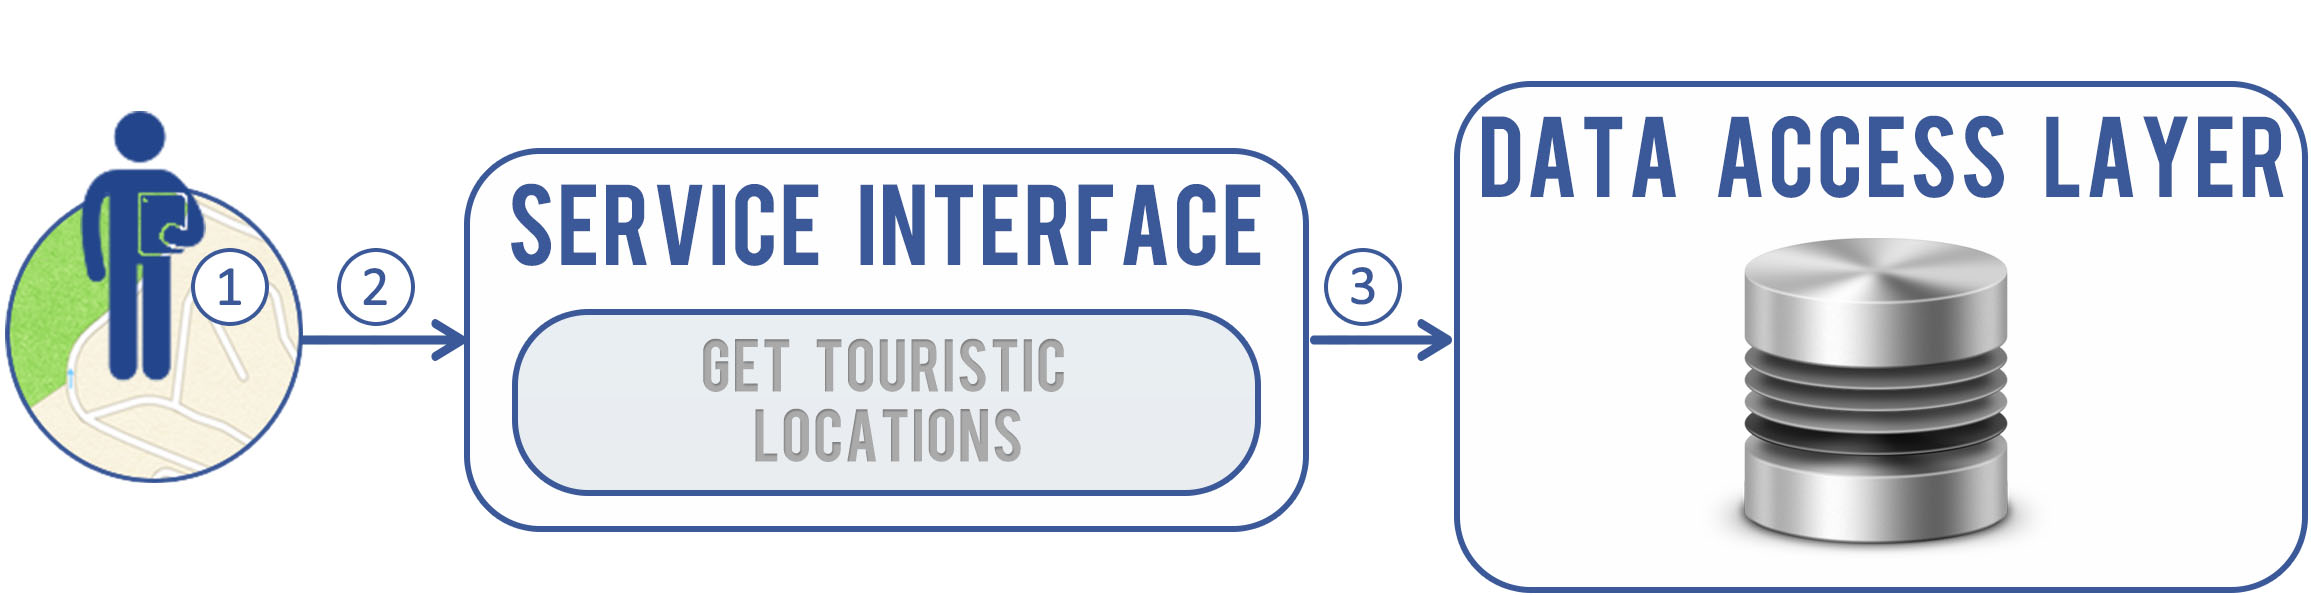
\includegraphics[width=13.0 cm]{./images/diagrams/diagram_usecase_users_location.jpg}
   \caption{Use-case of the near by feature.}
   \label{fig:useCaseFilterByLocation}
\end{figure}\\
%%%%%%%%%%%%%%%%%%%%
Each step is detailed as follows:
\begin{enumerate}
\item The geographic coordinates of user's current location, are obtained through the ~\gls{gps} of the mobile device.
\item Through the service interface, users make the requests to obtain the touristic locations passing the previously obtained geographic coordinates.
\item The service interface interacts with the Data Access Layer (DAL) in order to list the touristic locations. The distance is calculated between each sight and the submitted geographic coordinates, providing the results sorted in ascending order of distance.
\end{enumerate}
%%%%%%%%%%%%%%%%%%%%
The recommender system is one of the most important features of the developed service. The summarised process of the recommendation system is illustrated on Figure~\ref{fig:useCaseRecommendationLocation}.\\
%%%%%%%%%%%%%%%%%%%%
\begin{figure}[h!]
 \centering
   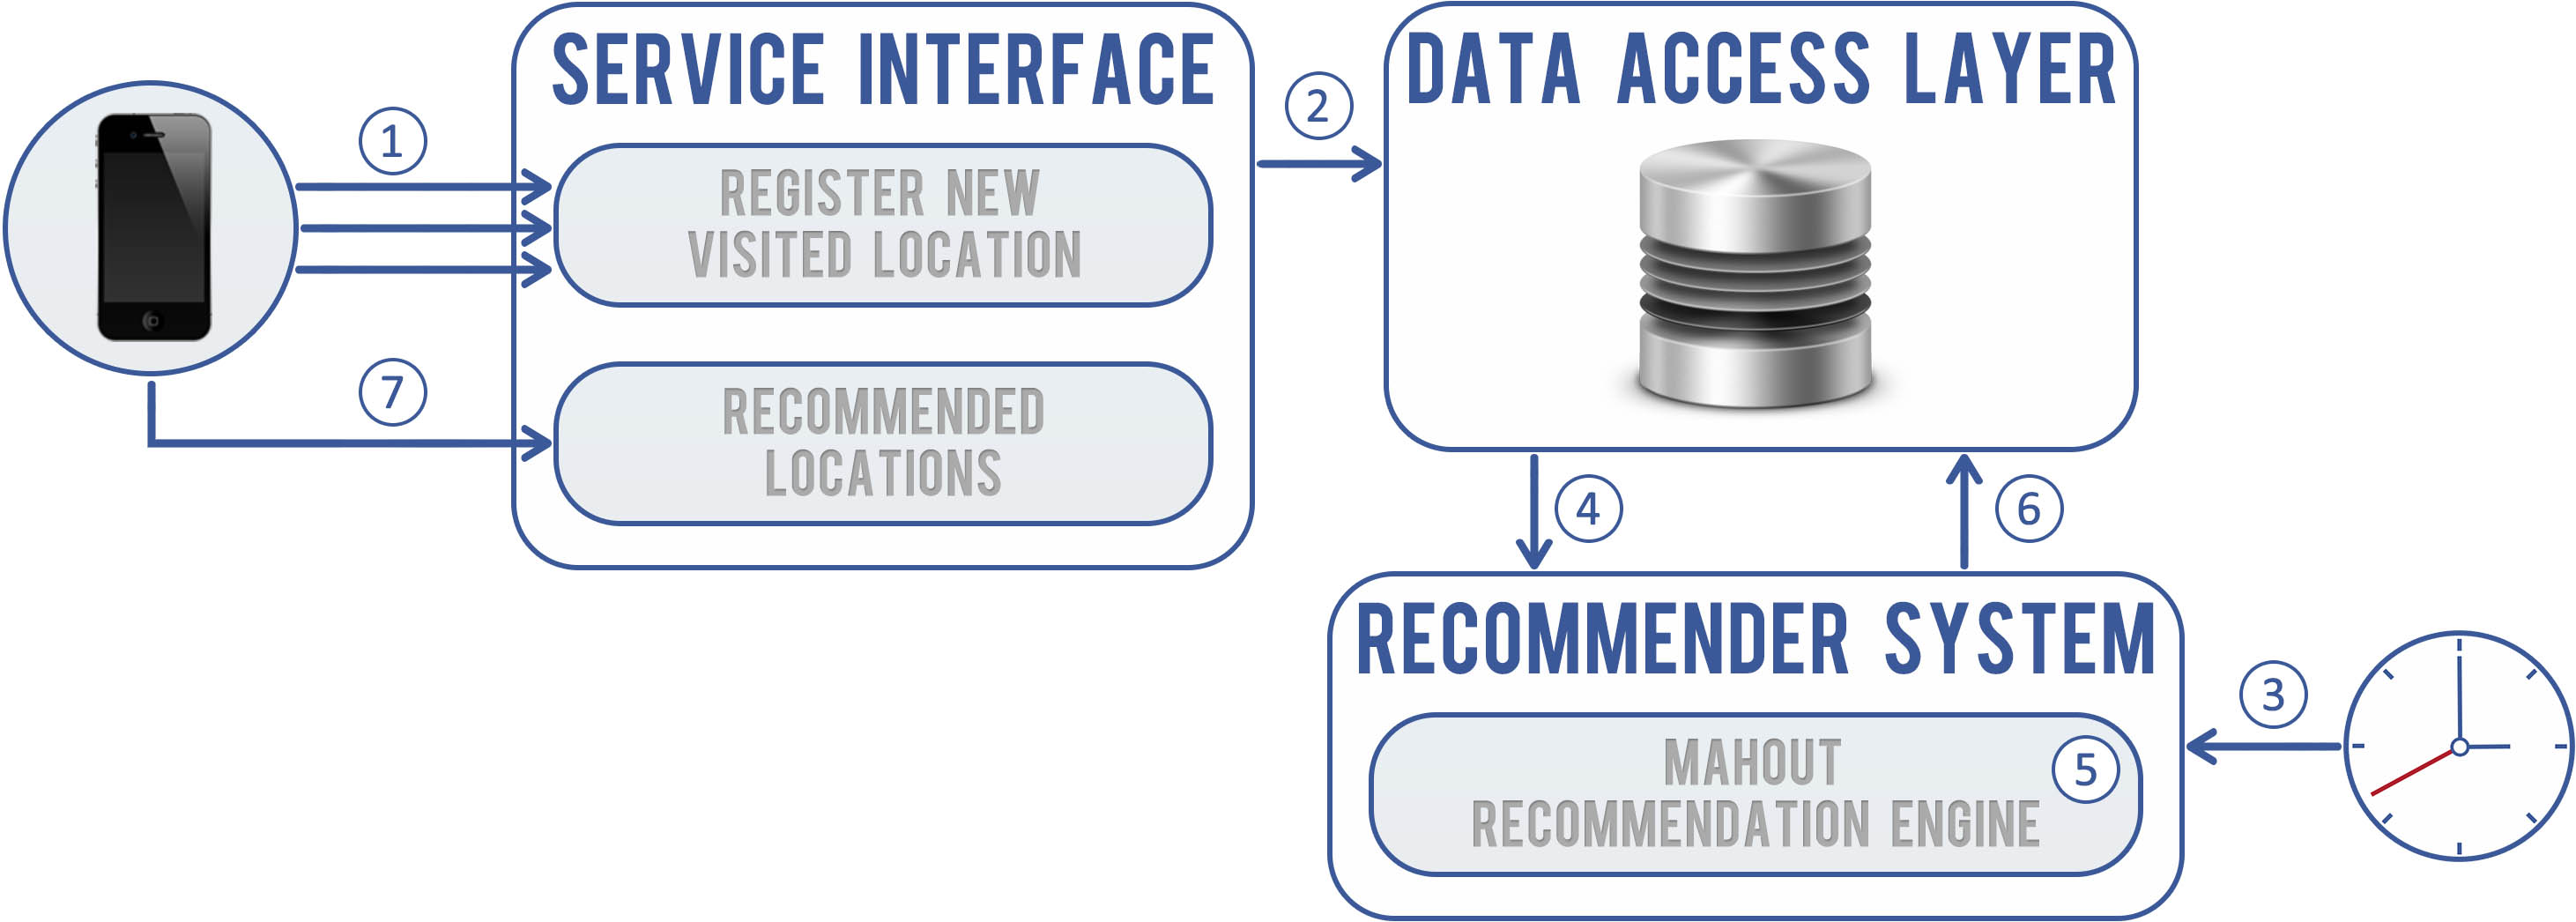
\includegraphics[width=13.0 cm]{./images/diagrams/diagram_usecase_recommender_system.jpg}
   \caption{The recommendation process.}
   \label{fig:useCaseRecommendationLocation}
\end{figure}\\
The full process of the recommendation system is as follows:
\begin{enumerate}
\item Through the service interface, the user marks new locations as visited.
\item Using the implemented DAL, the information is stored into the database.
\item The Cron Job\footnote{Cron is a time-based job scheduler in Unix-like computer operating systems.}~\cite{cronTab} is triggered everyday at 3:00 A.M., performing the recommendation process.
\item The recommender system obtains users eligible for the new recommendations.
\item For each user, the recommender system computes a set of locations previously unseen by the user.
\item Through the DAL, the recommender service removes previous recommendations and populates the database with the new information.
\item Later, the user obtains a list of recommendations through the service interface.
\end{enumerate}
%%%%%%%%%%%%%%%%%%%%
When comparing the GuideMe service with similar applications reviewed in Section~\ref{sec:sota}, it offers:
\begin{itemize}
	\item filters of unique kind that allow searching for points of interest;
	\item a friendly and usable interface for both Web and mobile applications;
	\item integration with algorithms and services that minimize human interaction during the approval process of newly inserted locations.
\end{itemize}

\section{Report Organization}
\label{sec:reportOrganization}
The remainder of this report is organized as follows. In Chapter~\ref{theory}, we introduce the background concepts and terminology of the recommender system and different collaborative filtering techniques. Chapter~\ref{implementation} approaches the proposed solution by detailing: the chosen service architecture, the integration with the~\gls{apns} service, the analysis of different frameworks for the implementation of the~\gls{dal}, and the~\gls{rest}~\gls{api}. Chapter~\ref{implementation} also includes prototypes that were initially designed before the development of the client applications.\\
\\
In Chapter~\ref{developed-work}, we describe all the developments that were made for making this project a reality. In detail, this Chapter describes the implementation aspects of the database models for both Service and Log databases, structure of the the~\gls{rest}~\gls{api} endpoints, different characteristics of the implemented recommender system, and push notification provider. We introduce the main features, as also some implementation details of the web and iOS applications. Chapter~\ref{chapter:expRsults} is devoted to the experimental results, which have guided the implementations in the correct direction. This Chapter reflects an analysis of the different recommendation system algorithms and load tests.\\
\\
We end the document with the Chapter~\ref{conclusions} by detailing the core aspects of the project and the fulfilled objectives. In order to make the service more usable and robust, as future work we present some points that should be improved in terms of security and functionalities.

\section{Our Contribution}
\label{sec:ourContribution}
We've recently submitted an article~\cite{guideMeArticle} to the 2013 Conference on Electronics, Telecommunications and Computers (CETC 2013), where we describe the main parts of this work. We believe that the developed project contribute to the evolution of tourist guide services, and promotes the effective integration of recommendation systems as a tool to easily find new interesting places to visit.
\fi
